\section{实验}

\subsection{实验设置}

全部代码在一组参数化的 Python 模块中实现（\texttt{report/code}）。表格方法与进化算法在 48 核服务器上多进程运行，DV-KM 在 RTX 3090 上训练，精确前沿用 HiGHS 求解。实验一共有 $6(\Dt)\times3(\text{车队})\times5(\text{种子})=90$ 个 Q-KM 训练任务。三种策略在相同的 10 个测试日上评估，测试日由测试期订单池生成，在各 $\Dt$ 与各策略之间共用，以便配对比较。显著性检验用双侧 Wilcoxon 符号秩检验：Q-KM 先对 5 个种子取均值，再与基线按测试日配对，$n=10$。表中 $^{*}$、$^{**}$、$^{***}$ 分别表示 $p<0.05$、$0.01$、$0.001$。

\subsection{实验一：多批次间隔下的收入对比}

\begin{figure*}[t]
	\centering
	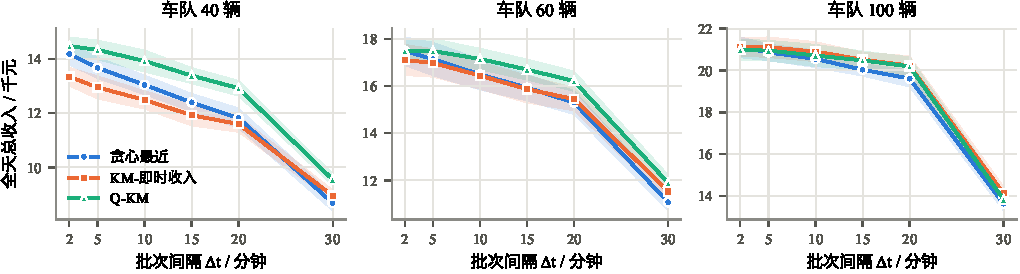
\includegraphics[width=\textwidth]{fig/exp1_revenue_dt.pdf}
	\caption{不同批次间隔 $\Dt$ 下三种策略的全天收入（10 个测试日均值，阴影为 95\% 置信区间）}
	\label{fig:exp1}
\end{figure*}

\begin{table}[t]
	\centering
	\caption{Q-KM 相对 KM 即时收入 / 最近贪心的收入增益（\%）}
	\label{tab:exp1gain}
	\small
	\setlength{\tabcolsep}{3.2pt}
	\begin{tabular}{c rr rr rr}
		\toprule
		& \multicolumn{2}{c}{40 辆} & \multicolumn{2}{c}{60 辆} & \multicolumn{2}{c}{100 辆} \\
		\cmidrule(lr){2-3}\cmidrule(lr){4-5}\cmidrule(lr){6-7}
		$\Dt$/min & vs KM & vs 贪心 & vs KM & vs 贪心 & vs KM & vs 贪心 \\
		\midrule
		\tabinput{tables/exp1_gain.tex}
		\bottomrule
	\end{tabular}
\end{table}

\begin{table}[t]
	\centering
	\caption{$\Dt=10$ min、60 辆车时的详细指标（10 个测试日均值；收入后为 95\% 置信区间半宽）}
	\label{tab:exp1detail}
	\small
	\setlength{\tabcolsep}{2.6pt}
	\resizebox{\columnwidth}{!}{\begin{tabular}{lccccc}
		\toprule
		策略 & 收入/元 & 送客/km & 应答率/\% & 接驾/km & 响应/min \\
		\midrule
		\tabinput{tables/exp1_detail.tex}
		\bottomrule
	\end{tabular}}
\end{table}

\Cref{fig:exp1} 和\cref{tab:exp1gain} 给出了 18 种设置下的结果，可以归纳出以下几点。

\textbf{(1) 运力越紧张，长期价值越重要。} 40 辆车时，Q-KM 相对 KM 即时收入在各 $\Dt$ 下增收 6.7\%–12.4\%，60 辆车时增收 2.4\%–5.4\%，均显著。100 辆车时，Q-KM 与 KM 的差距在 $\pm$2.1\% 以内，6 种设置中只有 2 种显著，而且都是 Q-KM 略低。此时验证集选出的 $\beta$ 均落在最小档 0.2–0.4，说明运力充足时到处都有空车，区域价值差异提供的信息很少。

\textbf{(2) KM 即时收入在运力紧张时不如最近贪心。} 40 辆、$\Dt=10$ 时，KM 即时收入为 \num{12494} 元，最近贪心为 \num{13050} 元。只看本批次车费的匹配偏向长途单，长途单把司机带离热点区域，空车又不会自行返回。Q-KM 的边权中包含 $\gamma V(t{+}1,i)$ 一项，代表“司机留在原地”的机会成本，这一缺陷由此得到修正（\cref{tab:exp1detail}：应答率从 59.0\% 升至 65.4\%）。

\textbf{(3) 批次间隔的影响。} 三种策略的收入都随 $\Dt$ 增大而单调下降，从 $\Dt=20$ 到 $\Dt=30$ 骤降 23\%–31\%。原因是订单耐心只有 20 分钟，比批次间隔还短，大量订单在下一批次执行前就已取消。另一方面，$\Dt$ 增大时 Q-KM 相对最近贪心的优势也在扩大（40 辆时从 2.1\% 升到 10.1\%）：批次越大，候选匹配越多，价值引导的选择余地也越大。$\Dt=2$–5 分钟时收入最高，平均响应时间（等待 + 接驾）也最短，是三者之间较好的折中。

\begin{figure*}[t]
	\centering
	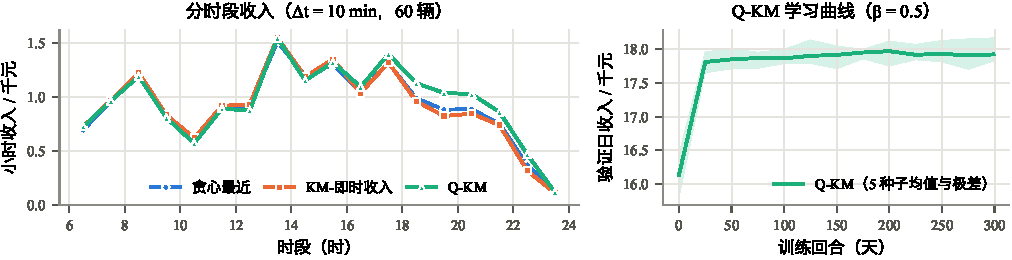
\includegraphics[width=\textwidth]{fig/exp1_hourly_curve.pdf}
	\caption{左：$\Dt=10$ min、60 辆车时按小时分解的收入；右：Q-KM 在验证日上的学习曲线（5 个种子）}
	\label{fig:hourly}
\end{figure*}

\textbf{(4) 收入从何而来。} 按小时分解（\cref{fig:hourly} 左）后可以看到，Q-KM 在 7:00–15:00 的收入反而比 KM 低 0.2\%–8.1\%：它会拒绝把司机派往冷区的高价订单，宁可让司机留在原地。到了 16:00 之后，Q-KM 的收入持续领先，18:00–22:00 时段高出 16\%–47\%。也就是说，Q-KM 的增益是\textbf{跨时段的}：白天保持车辆的空间分布，换来晚高峰更多的可用运力。批次级的贪心与 KM 只看当前批次，无法做出这种跨时段的取舍。学习曲线显示，训练约 25 个模拟日后验证收入即趋于稳定，最终验证收入在 5 个种子之间的极差约为 1.9\%。

\subsection{实验二：双目标帕累托前沿}

本节与拓展 A 共用同一组批次：8:00、13:00、18:00、23:00 各随机抽取 5 个批次，每批 40 个司机、80 个订单，距离量化到 10\,m。每个批次先用 \cref{sec:exact} 的方法求出精确前沿 $Z^\ast$，作为真值。三种进化算法各运行 5 个种子，加权和 KM 是确定性方法，只运行一次。所有指标都以 $Z^\ast$ 的理想点和最差点归一化：HV 比为 $\mathrm{HV}/\mathrm{HV}^\ast$，IGD 与 IGD$^+$ 越小越好，“命中率”指近似解中恰好落在 $Z^\ast$ 上的比例。

\begin{figure}[t]
	\centering
	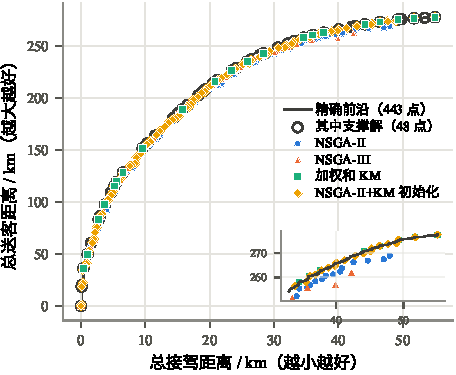
\includegraphics[width=\columnwidth]{fig/exp2_front.pdf}
	\caption{18:00 代表批次的帕累托前沿（右下为高收入端放大）。空心圆为精确前沿上的支撑解}
	\label{fig:front}
\end{figure}

\textbf{前沿形状与折中解。} \Cref{fig:front} 中，前沿在低接驾端很陡、在高收入端很平，边际收益递减明显。以与两端点连线距离最远的点（膝点）为折中方案，20 个批次平均只需最大接驾距离的 31.6\%，就能获得最大送客距离的 71.1\%。这说明平台若完全追求收入最大化，最后约 29\% 的收入需要付出约 68\% 的额外接驾距离。

\begin{table}[t]
	\centering
	\caption{近似算法对比（20 批次 × 5 种子均值；末列为以 IGD$^+$ 计的 Friedman 平均秩）}
	\label{tab:moo}
	\resizebox{\columnwidth}{!}{%
	\begin{tabular}{lccccccc}
		\toprule
		方法 & HV 比$\uparrow$ & IGD$\downarrow$ & IGD$^+\downarrow$ & Spacing$\downarrow$ & 解数 & 命中率/\% & 秩 \\
		\midrule
		\tabinput{tables/exp24_methods.tex}
		\bottomrule
	\end{tabular}}
\end{table}

\begin{figure}[t]
	\centering
	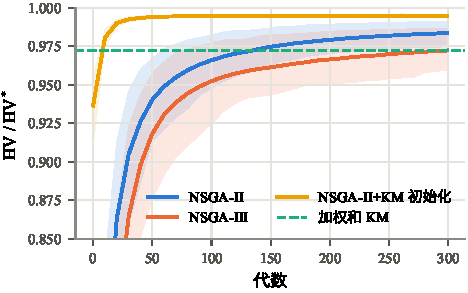
\includegraphics[width=\columnwidth]{fig/exp2_convergence.pdf}
	\caption{HV 比随代数的收敛（100 条曲线的均值，阴影为 10\%–90\% 分位）}
	\label{fig:conv}
\end{figure}

\textbf{算法比较。} 由\cref{tab:moo} 和\cref{fig:conv} 可以得到三点结论。(1) 两个目标时，NSGA-II 明显优于 NSGA-III：HV 比为 0.984 对 0.972，Spacing 为 0.47 对 0.84。NSGA-III 的参考方向在归一化目标空间中按角度均匀分布，而本问题的前沿弯曲程度很大，解会集中在少数方向上，拥挤距离反而能更好地适应局部密度。(2) 加权和 KM 每次都解到真正的最优，命中率达 98.9\%（未命中的点来自 $\lambda=0$ 时只最大化收入、接驾距离不唯一的弱支配解）。但它平均只找到 21.4 个点，HV 比仅 0.972，IGD$^+$ 是各方法中最差的。(3) KM 初始化把加权和 KM 的精确解作为“锚点”，NSGA-II 在锚点之间继续搜索非支撑解。这一做法使 HV 比提高到 0.995，IGD$^+$ 从 0.0071 降到 0.0033（约 54\%），命中率从 31\% 升到 55\%，并且在第 20 代左右就超过随机初始化 300 代的水平。

\textbf{统计检验。} 以 20 个批次为区组、IGD$^+$ 为指标做 Friedman 检验，$p=2.9\times10^{-11}$。四种方法的平均秩依次为 KM 初始化 1.0、NSGA-II 2.1、NSGA-III 3.2、加权和 3.7。Nemenyi 临界差 CD $=1.05$（$\alpha=0.05$），因此前三者两两之间差异显著，NSGA-III 与加权和之间不显著。配对 Wilcoxon 检验得到相同结论：KM 初始化对 NSGA-II，以及 NSGA-II 对加权和，均有 $p<10^{-5}$。

\subsection{拓展实验 A：精确前沿揭示的结构}

\begin{figure}[t]
	\centering
	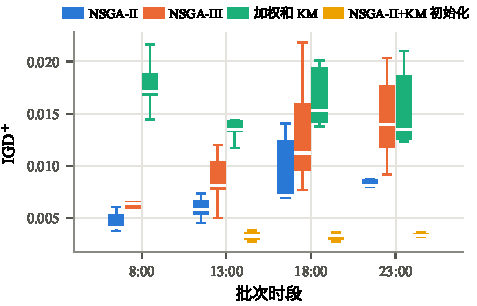
\includegraphics[width=\columnwidth]{fig/exp4_igd_hour.pdf}
	\caption{不同时段批次上各方法的 IGD$^+$（越小越好；每箱 5 个批次，每批取 5 个种子均值）}
	\label{fig:igdhour}
\end{figure}

20 个批次的精确前沿全部通过了 \cref{sec:exact} 中的逐点验证，修复次数为 0。每个批次平均有 445 个非支配点（306–593 个），平均需要求解 1335 次整数规划，点数最多的批次（593 点）在单进程下约需 3.4 分钟。主要发现如下：

\textbf{(1) 帕累托前沿以非支撑解为主。} 位于下凸包上的支撑解平均只有 43.5 个，占 \textbf{10.0\%}（各批次在 8.0\%–14.4\% 之间）。任何线性加权方法，无论 $\lambda$ 取得多密，都只能覆盖这约 10\% 的点。离散匹配问题的可行组合非常多，相邻的支撑解之间分布着大量“凹陷处”的折中解，这正是进化算法相对加权和方法的优势所在。此前的作业只把 HV 比作为评价依据，加权和 KM 与 NSGA-II 的 HV 比只差约 0.01，看起来接近。有了精确前沿，可以确认两者的差距真实存在，主要体现在前沿的覆盖率上（IGD$^+$ 相差 2.2 倍）。

\textbf{(2) 难度随时段变化。} \Cref{fig:igdhour} 中，18:00 和 23:00 批次的可行订单更多（平均 63 和 71 单，8:00 与 13:00 均约 59 单），前沿点更多，随机初始化的 NSGA-II/III 误差明显增大。KM 初始化在四个时段上的 IGD$^+$ 都稳定在 0.003 左右，对问题规模不敏感。

\textbf{(3) 对作业中“竞争比”的补充。} 若以精确前沿为基准，NSGA-II 找到的最高送客距离平均为 269.3\,km，比真实最大值 278.5\,km 低 3.3\%；而 KM 初始化与加权和 KM 都能达到真实最大值。可见随机初始化的进化算法在前沿两端收敛不足，用精确解作锚点可以弥补这一点。


\subsection{拓展实验 B：DV-KM 深度价值网络}

\begin{figure*}[t]
	\centering
	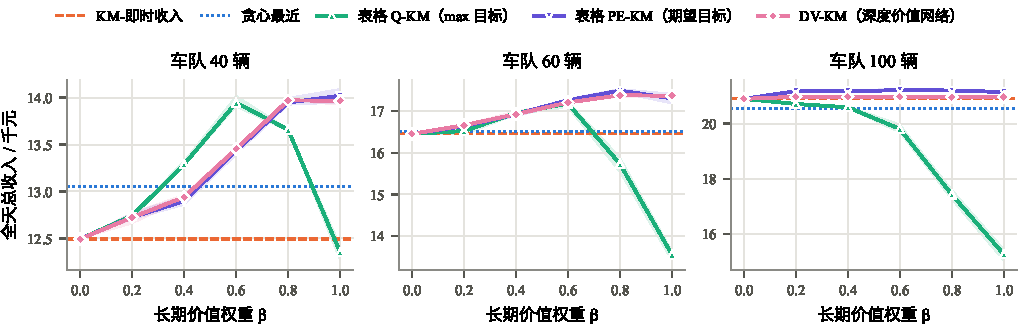
\includegraphics[width=\textwidth]{fig/exp3_beta.pdf}
	\caption{长期价值权重 $\beta$ 对全天收入的影响（$\Dt=10$ min，10 个测试日；阴影为 3 个训练种子的极差）}
	\label{fig:beta}
\end{figure*}

\begin{table*}[t]
	\centering
	\caption{各方法收入（元）。“最佳”列为测试集上的最佳 $\beta$（括号内，仅作上界参考），“$\beta=1$”列为 3 个种子的均值 $\pm$ 标准差}
	\label{tab:dvkm}
	\small
	\setlength{\tabcolsep}{6pt}
	{\begin{tabular}{l cc cc cc}
		\toprule
		& \multicolumn{2}{c}{40 辆} & \multicolumn{2}{c}{60 辆} & \multicolumn{2}{c}{100 辆} \\
		\cmidrule(lr){2-3}\cmidrule(lr){4-5}\cmidrule(lr){6-7}
		方法 & 最佳 & $\beta{=}1$ & 最佳 & $\beta{=}1$ & 最佳 & $\beta{=}1$ \\
		\midrule
		\tabinput{tables/exp3_main.tex}
		\bottomrule
	\end{tabular}}
\end{table*}

\Cref{fig:beta} 和\cref{tab:dvkm} 比较了三种价值估计方式，表格 PE-KM 用于分解两个因素的作用。

\textbf{max 目标是 $\beta$ 增大后收入崩溃的主因。} 表格 Q-KM 的收入在 $\beta=0.6$ 附近达到峰值，随后迅速下降。$\beta=1$ 时，60 辆和 100 辆车的收入分别只有 \num{13560} 元和 \num{15252} 元，比 KM 即时收入低 17.6\% 和 27.0\%，应答率从 0.79 跌到 0.63（100 辆）。同样是表格结构，把 TD 目标改成期望型的 PE-KM 后，收入随 $\beta$ 增大基本单调上升或保持平稳，$\beta=1$ 时为 \num{17302} 元和 \num{21145} 元。由此可以判断，崩溃来自 max 自举的过估计，而不是区域离散化。被高估的“原地等待”价值使大量正收益的边权变成负值，KM 便选择不派。拓展 D 将进一步说明，起作用的并不是高估的幅度，而是高估在“等待”与“出发”之间的不对称。

\textbf{深度网络带来鲁棒性，但没有带来更高的收入峰值。} DV-KM 在 3 个车队规模、6 个 $\beta$ 取值下都没有出现崩溃，$\beta=1$ 时种子间的标准差最小（23–56 元）。但它的最佳收入与表格 PE-KM 基本持平（40 辆 \num{13970} 对 \num{14019}，60 辆 \num{17376} 对 \num{17487}），100 辆时还低约 1.1\%。原因在于，本仿真中订单量与区域划分的比例使 $8\times8$ 表格的每个状态都有充足的样本，连续坐标的精细度没有可利用的空间。可以预期，在更细的空间粒度或样本更稀疏的城市中，函数逼近的泛化能力才会体现为收入优势。

\begin{table}[t]
	\centering
	\caption{DV-KM 消融（60 辆，同一份 175 万条经验，收入/元）}
	\label{tab:ablation}
	\small
	\setlength{\tabcolsep}{2.2pt}
	\begin{tabular}{lccccc}
		\toprule
		变体 \textbackslash\ $\beta$ & 0.2 & 0.4 & 0.6 & 0.8 & 1.0 \\
		\midrule
		\tabinput{tables/exp3_ablation.tex}
		\bottomrule
	\end{tabular}
\end{table}

\textbf{平滑正则是网络稳定的关键。} \Cref{tab:ablation} 中，用相同数据重新训练（仅随机初始化不同）引起的波动约 1.2\%；去掉粗编码后收入下降不超过 0.7\%，与这一波动处于同一量级。去掉平滑正则后，收入在 $\beta=0.4$ 时达到全表最高的 \num{17585} 元，但 $\beta\ge0.8$ 时跌回 \num{15744}/\num{14794} 元，与表格 Q-KM 的崩溃形态相同。缺少空间平滑时，网络在样本稀疏的位置会外推出虚高的价值，作用与 max 偏差类似。这与 CVNet\cite{tang2019deep}强调 Lipschitz 约束的动机一致。

\begin{figure*}[t]
	\centering
	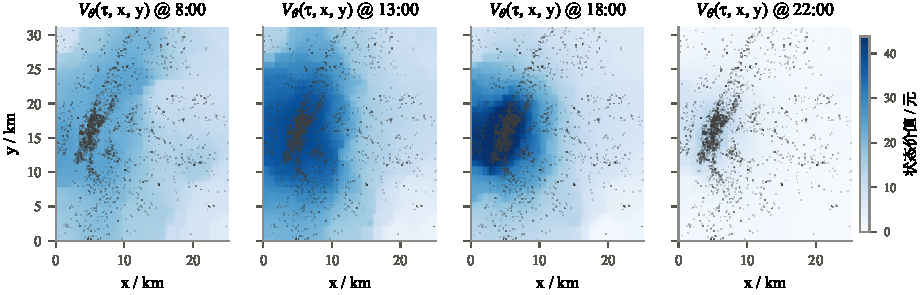
\includegraphics[width=0.92\textwidth]{fig/exp3_vmap.pdf}
	\caption{DV-KM 学到的连续价值函数 $V_\theta(\tau,x,y)$（60 辆车，灰点为训练期签到点）}
	\label{fig:vmap}
\end{figure*}

\Cref{fig:vmap} 展示了学到的价值面：13:00–18:00 曼哈顿中城与下城（$x\approx5$–10\,km，$y\approx12$–20\,km）的价值最高；8:00 时价值分布较分散，高值区尚未集中；22:00 整体价值趋近于 0，因为营业即将结束，剩余可赚的时间很短。价值面在空间上连续平滑，没有表格方法在网格边界处的阶跃。

\subsection{拓展实验 C：离事后最优还有多远}

\begin{table*}[t]
	\centering
	\caption{事后最优区间与在线策略（5 个测试日均值，与实验一配对）。“KM”“Q-KM”列为收入占 LB 的百分比；“弥合”为 Q-KM 弥合的 (LB$-$KM) 缺口比例。$^\dagger$：该设置有 4 天 MILP 在 400\,s 内未收敛，只报 UB，比例以 UB 为分母（是达成率的下界）}
	\label{tab:hindsight}
	\small
	\setlength{\tabcolsep}{5pt}
	{\begin{tabular}{c cccc cccc cccc}
		\toprule
		& \multicolumn{4}{c}{40 辆} & \multicolumn{4}{c}{60 辆} & \multicolumn{4}{c}{100 辆} \\
		\cmidrule(lr){2-5}\cmidrule(lr){6-9}\cmidrule(lr){10-13}
		$\Dt$ & [LB, UB]/千元 & KM & Q-KM & 弥合 & [LB, UB]/千元 & KM & Q-KM & 弥合 & [LB, UB]/千元 & KM & Q-KM & 弥合 \\
		\midrule
		\tabinput{tables/exp5.tex}
		\bottomrule
	\end{tabular}}
\end{table*}

\Cref{tab:hindsight} 给出了 \cref{sec:hindsight} 的事后最优区间。LB 是一个可执行的事后计划，因而真实的事后最优不低于 LB；表中以 LB 为分母的达成率因此是\textbf{偏乐观的}，在线策略离最优的实际差距只会更大。除 100 辆、$\Dt=10$ 外，所有 LB 都由 MILP 求到最优，回放仿真器后收入与 LB 逐日一致。

\textbf{运力紧张、批次较密时，短视的代价最大。} $\Dt=10$ 时，即使只用接驾按最坏情况计的保守计划，事后也能拿到 \num{17416} 元（40 辆）和 \num{20602} 元（60 辆）。KM 即时收入只达到其中的 71\% 和 81\%，Q-KM 达到 81\% 和 85\%，即 Q-KM 弥合了 KM 与事后最优之间 33\% 和 18\% 的缺口。这说明 Q-KM 的长期价值确实把策略推向了离线最优的方向，但仍有至少 15\%–19\% 的收入因不知道未来而损失；若以 UB 计，Q-KM 只达到 73\%/79\%。100 辆车时 KM 已达到 UB 的 87\%，Q-KM 没有额外收益，与实验一中“运力充足时长期价值无用”的结论一致。

\textbf{大批次间隔下的损失主要是结构性的。} $\Dt$ 从 10 增大到 30 分钟，事后最优本身就下降约三分之一（40 辆的 LB 从 \num{17416} 降至 \num{11407} 元，60 辆从 \num{20602} 降至 \num{13425} 元）。此时上下界只相差 4\%–5\%，在线策略的达成率反而升高到 80\%–93\%。也就是说，实验一中 $\Dt=30$ 时的收入骤降，大部分是“订单在下一批次前就已取消”造成的，即便事先知道全部订单也无法挽回，并不是派单算法的失误。批次间隔这一\textbf{系统设计参数}，比在给定间隔下改进匹配算法更重要。


\subsection{拓展实验 D：崩溃的根源是“等待被高估”}

\begin{figure*}[t]
	\centering
	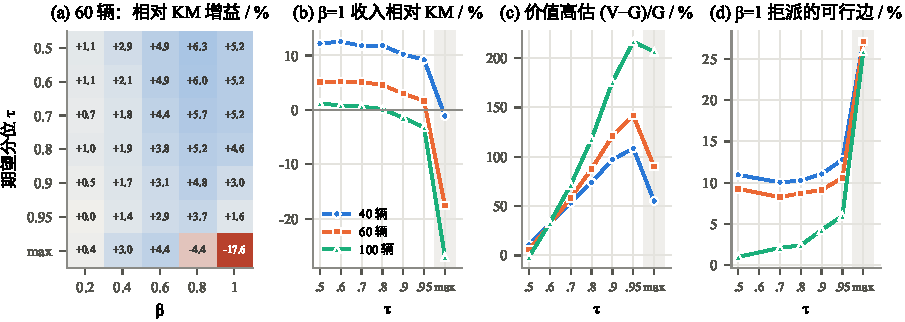
\includegraphics[width=\textwidth]{fig/exp6_expectile.pdf}
	\caption{价值目标乐观度谱（$\Dt=10$ min，3 个训练种子 × 10 个测试日）。(a) 60 辆车时各 $(\tau,\beta)$ 相对 KM 即时收入的增益；(b) $\beta=1$ 时的收入；(c) 价值表相对真实折扣回报的高估（$\beta=0.6$ 策略）；(d) $\beta=1$ 派单时边权 $\le0$、被拒派的可行边比例。灰色区域为 max 目标}
	\label{fig:expectile}
\end{figure*}

\begin{table}[t]
	\centering
	\caption{$\beta=1$ 时可行边上的平均价值项（元，3 种子 × 5 测试日）}
	\label{tab:gostay}
	\small
	\setlength{\tabcolsep}{3pt}
	\begin{tabular}{llcccc}
		\toprule
		车队 & 目标 & 出发 & 等待 & 出发$-$等待 & 出发/等待 \\
		\midrule
		\tabinput{tables/exp6b.tex}
		\bottomrule
	\end{tabular}
\end{table}

拓展 B 把 Q-KM 的崩溃归因于 max 目标的过估计。如果这一解释成立，那么任何足够乐观的目标都应当同样崩溃。\Cref{fig:expectile} 用期望分位目标检验了这个推论，结果与之相反。

\textbf{高估的幅度不能解释崩溃。} 随着 $\tau$ 增大，价值表的高估单调上升（\cref{fig:expectile}(c)）。$\tau=0.95$ 时高估达到 109\%/142\%/217\%（40/60/100 辆），与 max 目标的 55\%/90\%/206\% 相当，甚至更高。但 $\tau=0.95$ 在 $\beta=1$ 时的收入仍为 KM 的 $+9.2$\%/$+1.6$\%/$-3.2$\%，而 max 目标是 $-1.1$\%/$-17.6$\%/$-27.0$\%（\cref{fig:expectile}(b)）。在各自最佳的 $\beta$ 下，$\tau$ 从 0.5 增大到 0.95 只让增益平滑地下降 1.2–2.5 个百分点，热力图上也看不到 max 目标在右下角出现的断崖（\cref{fig:expectile}(a)）。

\textbf{决定性的是高估落在哪里。} \Cref{tab:gostay} 把边权中的长期项拆成“出发”$\gamma^{\Delta}V(t{+}\Delta,k)$ 与“等待”$\gamma V(t{+}1,i)$。期望分位目标把两者近似同比例放大：$\tau$ 从 0.5 到 0.95，出发/等待之比始终在 0.88–0.93 之间，因而在边权的差分中大部分相互抵消。max 目标则不同：与 $\tau=0.95$ 相比，它的出发价值低 5.8–10.9 元，等待价值只低 0.1–7.0 元，出发/等待之比降到 0.84，长期项从 PE 的 $-2.3$ 至 $-6.4$ 元扩大到 $-11.7$ 至 $-12.3$ 元。结果有 26\%–27\% 的可行边被判为负权而不派（\cref{fig:expectile}(d)），而期望分位目标下这一比例不超过 13\%。

\textbf{一个解释：max 的乐观按决策时点累积。} Q-learning 的目标在每个决策时点对 $\mathcal{A}(s')\cup\{\text{等待}\}$ 取一次 max，等于假设司机下一时刻总能接到附近最好的订单。原地等待的司机每 10 分钟就经历一个决策时点，送客的司机在 $\Delta$ 个时间片里只在到达时经历一次。因此单位时间内，等待状态积累的乐观远多于出发状态，平台被系统性地诱导去“等更好的单”。期望分位的乐观则作用在每次更新所采样的回报上，等待转移的回报几乎是确定的（无收入、仍在原区域），不会因决策时点多而额外放大。这一解释与\cref{tab:gostay} 中“max 只压低出发/等待之比”的现象一致，但严格验证还需要控制决策频率的对照实验。这一结论说明，改进长期价值派单的关键不在于压低价值的整体水平，而在于保证不同动作之间的\textbf{相对}价值无偏。


\subsection{拓展实验 E：批次级权衡在全天是否成立}

\begin{figure*}[t]
	\centering
	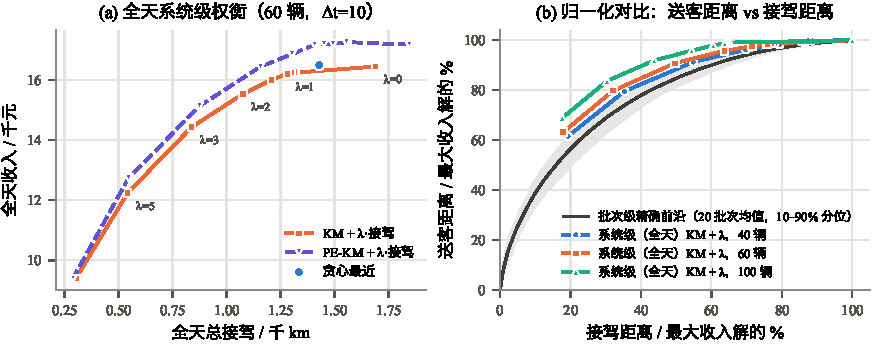
\includegraphics[width=\textwidth]{fig/exp7_system_front.pdf}
	\caption{(a) 在 KM / PE-KM 边权中加入接驾惩罚 $\lambda\cdot2p_{dj}$ 后的全天收入–总接驾距离（10 个测试日均值）；(b) 以最大收入解为 100\% 归一化后，批次级精确前沿与全天系统级曲线的对比}
	\label{fig:system}
\end{figure*}

实验二与拓展 A 都在单个批次内讨论“收入–接驾”的权衡。但平台真正关心的是全天累计的指标，单批次的前沿是否反映系统层面的代价，需要另行检验。为此在全天仿真中把边权改为 $w_{dj}=\text{fare}_j-\lambda\cdot2p_{dj}$（$\lambda=1$ 表示 1\,km 接驾与 1\,km 送客等价），扫描 $\lambda\in[0,8]$，分别作用于 KM 即时收入和表格 PE-KM（$\beta=0.6$），$\Dt\in\{5,10,20\}$，三种车队。

\textbf{全天层面的权衡远比单批次平缓。} \Cref{fig:system}(b) 中，三条全天曲线都位于批次级精确前沿的上方。在单个批次内，把接驾距离压缩 20\% 平均要损失 3.0\% 的送客距离，压缩 35\% 要损失 7.7\%。在全天层面，KM 只需取 $\lambda=0.25$，接驾总距离就下降 12\%/22\%/35\%（40/60/100 辆），而收入只变化 $-0.0$\%/$-1.2$\%/$-1.1$\%。换成 PE-KM，同一 $\lambda$ 下接驾下降 11\%–25\%，收入反而上升 0.1\%–0.5\%；40 辆车、$\lambda=0.5$ 时收入上升 1.0\%。$\Dt=5$ 与 20 分钟时结论相同：在全部 12 种（$\Dt$，车队，基础策略）组合下，$\lambda=0.25$ 使接驾下降 8\%–35\%，收入变化在 $-1.2$\% 至 $+0.5$\% 之间。直到 $\lambda\ge2$，即接驾惩罚开始切断大量正收益的边，收入才明显下降（$\lambda=2$ 时 $-4$\% 至 $-6$\%，$\lambda=3$ 时 $-10$\% 至 $-13$\%）。

\textbf{原因是批次之间的替代与运力回收。} 单批次前沿假设“这一批没派的订单就丢了”。但订单耐心（20 分钟）不短于批次间隔，被远处司机放弃的订单往往在本批次由近处司机接走，或在下一批次被其他司机服务，批次级的收入损失大部分在后续批次中被收回。另一方面，接驾时间本身占用运力：缩短接驾使司机更早空闲，在运力紧张时直接转化为更多的服务单量。这与网约车经济学中“空驶追单”（wild goose chase）的论断一致\cite{castillo2017surge}。最近贪心在 60/100 辆时接驾距离比 KM 短 15\%/34\%，收入差距却在 $\pm$1.7\% 以内，也印证了这一点。

由此得出一个实际的结论：以批次级帕累托前沿上的代价来权衡乘客体验和平台收入，会把真实代价\textbf{高估数倍}。在本仿真中，存在一段近乎“免费”的区间（$\lambda\approx0.25$–1），可以显著缩短接驾而几乎不损失收入。多目标派单应在系统层面评估，而不仅仅在单个批次上求前沿。

